\documentclass{article}
\usepackage{fullpage}
\usepackage{graphicx}
\usepackage{amsmath}
\usepackage{mathtools}
\usepackage{xcolor}
\usepackage{bm}
\usepackage{natbib}
\usepackage[hidelinks]{hyperref}
\usepackage{doi}
\usepackage{charter}
\usepackage[bitstream-charter]{mathdesign}
\usepackage[final,babel]{microtype}
\usepackage[utf8]{inputenc}
\usepackage[british]{babel}
\usepackage{csquotes}
\usepackage[T1]{fontenc}
\usepackage{siunitx}
\usepackage[font={small}]{caption}


\title{Multidimensional advection over steep terrain on a new type of Cartesian mesh \\ \TODO{(working title)}}
\author{James Shaw}

\newcommand{\iu}{{i\mkern1mu}}
\newcommand{\iunit}{\boldsymbol{\hat \imath}}
\newcommand{\junit}{\boldsymbol{\hat \jmath}}
\newcommand{\kunit}{\boldsymbol{\hat k}}
\newcommand{\TODO}[1]{\textcolor{purple}{TODO: \emph{#1}}}

\begin{document}
\maketitle

\section{Introduction}

First, we present a multidimensional advection scheme that is computationally cheap and suitable for complex flows on arbitrary meshes.  Second, we present a new type of Cartesian mesh, the slanted cell mesh, that avoids the small cell problem associated with cut cell meshes.   We apply the advection scheme to tests over steep orography and show that accurate results are obtained on slanted cell meshes.  Finally, we challenge the multidimensional advection scheme using a test of deformational flow on a geodesic mesh.

\section{Slanted cell mesh generation}

\TODO{can slanted cells represent cliffs?  Terry is keen to do tests with cliffs.  \citet{yamazaki-satomura2010} did tests with cliffs, too.}

\begin{figure}
	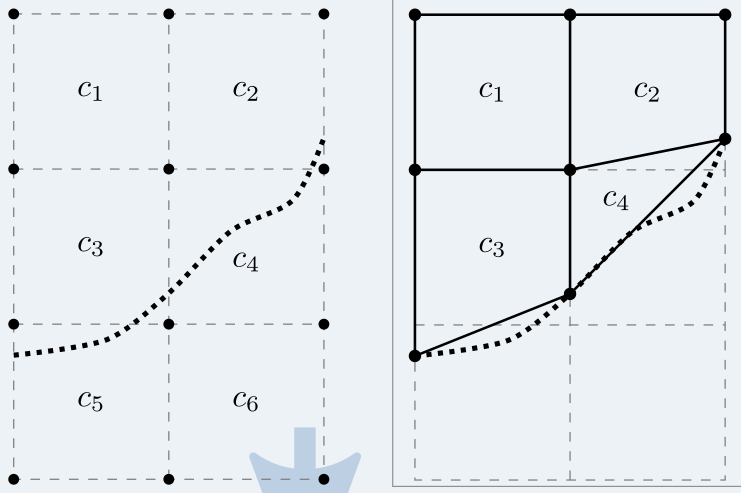
\includegraphics[width=0.5\textwidth]{slantCellConstruction.png}
	\caption{\TODO{Before and after diagrams showing how a slanted cell mesh is constructed from a uniform quadrilateral mesh}}
\end{figure}

\begin{figure}
	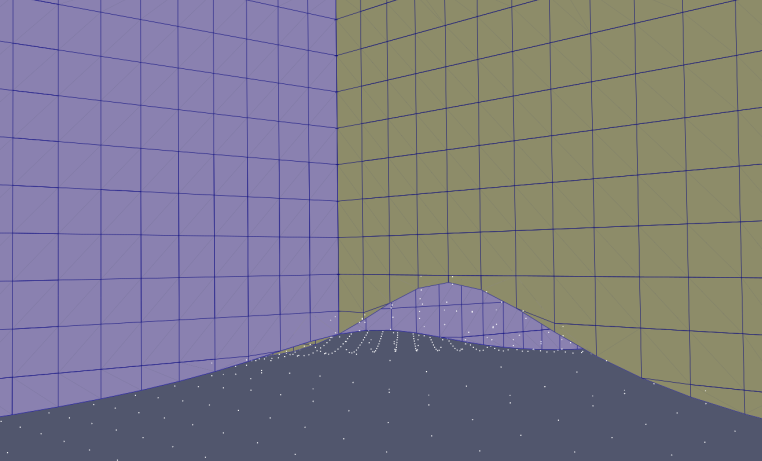
\includegraphics[width=0.5\textwidth]{3dslices.png}
	\caption{\TODO{An example of a 3D slanted cell mesh with Alpine topography, maybe best illustrated using orthogonal cross-sections.  Can we show this for triangles, quads and hexagons in the horizontal?}}
\end{figure}

\begin{figure}
	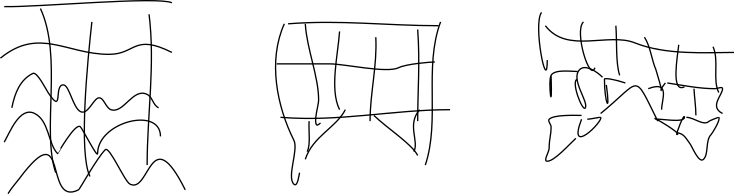
\includegraphics[width=\textwidth]{meshComparison.png}
	\caption{\TODO{examples of BTF, slanted cell and cut cell meshes with the same steep mountain profile (one of those used in the thermal advection test)}}
\end{figure}

\clearpage

\section{Multidimensional advection scheme}

The advection of a dependent variable $\phi$ is given by the conservation equation
\begin{align}
	\frac{\partial \phi}{\partial t} + \nabla \cdot \left( \mathbf{u} \phi \right) = 0 \label{eqn:advection}
\end{align}
where $\mathbf{u}$ is a prescribed wind field.  The time derivative is discretised using a three-stage, second-order Runge-Kutta scheme:
\begin{subequations}
\begin{align}
	\phi^\star &= \phi^{(n)} + \Delta t f(\phi^{(n)}) \\
	\phi^{\star\star} &= \phi^{(n)} + \frac{\Delta t}{2} \left( f(\phi^{(n)}) + f(\phi^\star) \right) \\
	\phi^{(n+1)} &= \phi^{(n)} + \frac{\Delta t}{2} \left( f(\phi^{(n)}) + f(\phi^{\star\star}) \right)
\end{align}
\end{subequations}
where \(f(\phi^{(n)}) = - \nabla \cdot (\mathbf{u} \phi^{(n)})\) at time level \(n\).

Using the finite volume method, the wind field is prescribed at face centroids and the dependent variable is stored at cell centroids.  The divergence term in equation~\eqref{eqn:advection} is discretised using Gauss's theorem:
\begin{align}
	\nabla \cdot \left( \mathbf{u} \phi \right) \approx \frac{1}{\mathcal{V}_c} \sum_{f \in c} \mathbf{u}_f \cdot \mathbf{S}_f \phi_F
\end{align}
where $\mathcal{V}_c$ is the cell volume, $\mathbf{u}_f$ is a wind vector prescribed at a face, ${\mathbf{S}_f}$ is the surface area vector with a direction outward normal to the face and a magnitude equal to the face area, and $\sum_{f \in c}$ denotes a summation over all faces $f$ belonging to cell $c$.  The value of the dependent variable at the face, $\phi_F$, is approximated by a least squares fit over a stencil of surrounding cell centre values.

\begin{figure}
	\centering
	\includegraphics{../fig-upwind-stencil/fig-upwind-stencil.pdf}
	\caption{Upwind-biased stencils for faces far away from the boundaries of two-dimensional (a) triangular, (b) rectangular and (c) hexagon meshes.  The stencil is used to fit a multidimensional polynomial to cell centre values, $\phi_c$, marked by grey circles, in order to approximate the value $\phi_F$ at the face centroid marked by an open circle.  $\phi_u$ and $\phi_d$ are the values at the centroids of the upwind and downwind cells neighbouring the target face, drawn with a heavy line.  The wind vector $\mathbf{u}_f$ is prescribed at face $f$ and determines the choice of stencil at each timestep.}
	\label{fig:interiorStencils}
\end{figure}

To introduce the approximation method, we will consider how an approximate value is calculated for a face that is far away from the boundaries of a two-dimensional uniform rectangular mesh.  For any mesh, every interior face connects two adjacent cells.  The wind direction at the face determines which of the two adjacent cells is the upwind cell.  Since the stencil is upwind-biased, two stencils must be constructed for every interior face, and the appropriate stencil is chosen for each face depending on the wind direction at that face for every timestep.

The upwind-biased stencil for a face $f$ is shown in figure~\ref{fig:interiorStencils}b.  The wind at the face, $\mathbf{u}_f$, is blowing from the upwind cell $c_u$ to the downwind cell $c_d$.
To obtain an approximate value at $f$, a polynomial least squares fit is calculated using the stencil values.
The stencil has \num{4} points in $x$ and \num{3} points in $y$, leading to a natural choice of polynomial that is cubic in $x$ and quadratic in $y$:
\begin{align}
	\phi = a_1 + a_2 x + a_3 y + a_4 x^2 + a_5 xy + a_6 y^2 + a_7 x^3 + a_8 x^2 y + a_9 x y^2 \label{eqn:fullPoly}
\end{align}
A least squares approach is needed because the system of equations is overconstrained, with \num{12} stencil values but only \num{9} polynomial terms.  If the stencil geometry is expressed in a local coordinate system with the face centroid as the origin, then the approximated value $\phi_F$ is equal to the constant term $a_1$.

The remainder of this section generalises the the approximation technique for arbitrary meshes, explaining the methods for constructing stencils, performing a least squares fit with a suitable polynomial, and ensuring numerical stability of the advection scheme.

\subsection{Stencil construction}
For every interior face, two stencils are constructed, one for each of the possible upwind cells.  For a given face $f$ and upwind cell $c_u$, we find those faces that are connected to $c_u$ and `oppose' face $f$.  These are called the \textit{opposing faces}.
The opposing faces for face $f$ and upwind cell $c_u$ are determined as follows.
Defining $G$ to be the set of other faces bounding cell $c_u$, we calculate the `opposedness', $\mathrm{Opp}$, between faces $f$ and $g \in G$, defined as
\begin{align}
	\mathrm{Opp}(f, g) \equiv - \frac{\mathbf{S}_f \cdot \mathbf{S}_g}{|\mathbf{S}_f|^2} \label{eqn:opp}
\end{align}
where $\mathbf{S}_f$ and $\mathbf{S}_g$ are the surface area vectors pointing outward from cell $c_u$ for faces $f$ and $g$ respectively.
Using the fact that $\mathbf{a} \cdot \mathbf{b} = |\mathbf{a}|\:|\mathbf{b}| \cos(\theta)$ we can rewrite equation~\eqref{eqn:opp} as
\begin{align}
	\mathrm{Opp}(f, g) = - \frac{|\mathbf{S}_g|}{|\mathbf{S}_f|} \cos(\theta)
\end{align}
where $\theta$ is the angle between faces $f$ and $g$.  In this form, it can be seen that $\mathrm{Opp}$ is a measure of the area of $g$ and how closely it parallels face $f$.

The set of opposing faces, $\mathrm{OF}$, is a subset of $G$, comprising those faces with $\mathrm{Opp} \geq 0.5$, and the face with the maximum opposedness.  Expressed in set notation, this is
\begin{align}
	\mathrm{OF}(f,c_u) \equiv \{ g : \mathrm{Opp}(f, g) \geq 0.5 \} \cup \{ g : \max(\mathrm{Opp}(f, g)) \} 
\end{align}
On a two-dimensional rectangular mesh, there is always one opposing face that is exactly parallel to the face $f$.

Once the opposing faces have been determined, the set of internal and external cells must be found.  The \textit{internal cells} are those cells that are connected to the opposing faces.  Note that $c_u$ is always an internal cell.  The \textit{external cells} are those cells that share vertices with the internal cells.  Note that $c_d$ is always an external cell.  Having found these two sets of cells, the stencil is constructed to comprise all internal and external cells.

\begin{figure}
	\centering
	\includegraphics{../fig-double-upwind-stencil/fig-double-upwind-stencil.pdf}
	%
	\caption{A thirteen-cell, upwind-biased stencil for face $f$ connecting the pentagonal upwind cell, $c_u$, and the downwind cell $c_d$.  The dashed lines denote the two faces of cell $c_u$ that oppose $f$, and black circles mark the centroids of the internal cells that are connected to these two opposing faces.  The stencil is extended outwards by including cells that share vertices with the three internal cells, where black squares mark these vertices.  The local coordinate system $(x, y)$ has its origin at the centroid of face $f$, marked by an open circle, with $x$ normal to $f$ and $y$ perpendicular.}
	\label{fig:double-upwind-stencil}
\end{figure}

Figure~\ref{fig:double-upwind-stencil} illustrates a stencil construction for face $f$ connecting upwind cell $c_u$ and downwind cell $c_d$.  The two opposing faces are denoted by thick dashed lines and the centres of the three adjoining internal cells are marked by black circles.  The stencil is extended outwards by including the external cells that share vertices with the internal cells, marked by black squares.  The resultant stencil contains 13 cells.


\subsection{Least squares fit}
To approximate the value at a face $f$, a least squares fit is calculated from a stencil of surrounding cell centre values.  First, we will show how a polynomial least squares fit is calculated for a face on a rectangular mesh.  Second, we will make modifications to the least squares fit that are necessary for numerical stability.  Finally, we will describe how the approach is applicable to faces of arbitrary meshes.  

For faces that are far away from the boundaries of a rectangular mesh, we fit the multidimensional polynomial given by equation~\eqref{eqn:fullPoly} that has nine unknown coefficients, $\mathbf{a} = a_1 \ldots a_9$, using the twelve cell centre values from the upwind-biased stencil, $\bm{\phi} = \phi_1 \ldots \phi_{12}$.  This yields a matrix equation
\begin{align}
	\begin{bmatrix}
		1 & x_1 & y_1 & x_1^2 & x_1 y_1 & y_1^2 & x_1^3 & x_1^2 y_1 & x_1 y_1^2 \\
		1 & x_2 & y_2 & x_2^2 & x_2 y_2 & y_2^2 & x_2^3 & x_2^2 y_2 & x_2 y_2^2 \\
		\vdots & \vdots & \vdots & \vdots & \vdots & \vdots & \vdots & \vdots & \vdots \\
		1 & x_{12} & y_{12} & x_{12}^2 & x_{12} y_{12} & y_{12}^2 & x_{12}^3 & x_{12}^2 y_{12} & x_{12} y_{12}^2 \\
	\end{bmatrix}
	\begin{bmatrix}
		a_1 \\
		a_2 \\
		\vdots \\
		a_9
	\end{bmatrix}
	=
	\begin{bmatrix}
		\phi_1 \\
		\phi_2 \\
		\vdots \\
		\phi_{12}
	\end{bmatrix}
\end{align}
which can be written as
\begin{align}
	\mathbf{B} \mathbf{a} = \bm{\phi} \label{eqn:unweightedLeastSquares}
\end{align}
The rectangular matrix $\mathbf{B}$ has one row for each cell in the stencil and one column for each term in the polynomial.  $\mathbf{B}$ is constructed using only the mesh geometry and is called the \textit{stencil matrix}.
A local coordinate system is established in which $x$ is normal to the face $f$ and $y$ is perpendicular to $x$.
The coordinates $(x_i, y_i)$ give the position of the centroid of the $i$th cell in the stencil.
The unknown coefficients $\mathbf{a}$ are calculated using the pseudo-inverse of $\mathbf{B}^+$ found by singular value decomposition:
\begin{align}
	\mathbf{a} = \mathbf{B}^+ \bm{\phi}
%
\intertext{Recall that the approximate value $\phi_F$ is equal to the constant coefficient $a_1$, which is calculated as} 
%
	a_1 = \begin{bmatrix}
		b_{1,1}^+ \\
		b_{1,2}^+ \\
		\vdots \\
		b_{1,12}^+
	\end{bmatrix}
	\cdot
	\begin{bmatrix}
		\phi_1 \\
		\phi_2 \\
		\vdots \\
		\phi_{12}
	\end{bmatrix}
\end{align}
where $b_{1,1}^+ \ldots b_{1,12}^+$ are the elements of the first row of $\mathbf{B}^+$.

The least squares fit presented above was unweighted, with equal weight placed on all stencil cell values.  \citet{lashley2002} showed that a weighted least squares fit is necessary for numerical stability, with greater weight being placed on the cells connected to face $f$.  We assign a weight to each stencil value, $\mathbf{w} = w_1 \ldots w_{12}$ and multiply by equation~\eqref{eqn:unweightedLeastSquares} to obtain
\begin{align}
	\mathbf{\tilde{B}} \mathbf{a} = \mathbf{w} \cdot \bm{\phi}
\end{align}
where $\mathbf{\tilde{B}} = \mathbf{W} \mathbf{B}$ and $\mathbf{W} = \mathrm{diag}(\mathbf{w})$.  The constant coefficient $a_1$ is calculated from the pseudo-inverse, $\mathbf{\tilde{B}}^+$:
\begin{align}
	a_1 = \mathbf{\tilde{b}_1^+} \cdot \mathbf{w} \cdot \mathbf{\phi}
\end{align}
where $\mathbf{\tilde{b}_1^+} = \tilde{b}_{1,1}^+ \ldots \tilde{b}_{1,12}^+$ are the elements of the first row of $\mathbf{\tilde{B}}^+$.

For faces of a non-rectangular mesh, or faces that are near a boundary, the number of stencil cells and number of polynomial terms may differ: a stencil will have two or more cells and, for two-dimensional meshes, its polynomial will have between one and nine terms.  Additionally, the polynomial cannot have more terms than its stencil has cells because this would lead to an underconstrained system of equations.  The procedure for choosing suitable polynomials is discussed next.

\subsection{Polynomial generation}
\begin{figure}
	\centering
	\caption{\TODO{2x3 and 3x3 meshes}}
	\label{fig:boundaryStencils}
\end{figure}

The majority of faces on a uniform two-dimensional mesh have stencils with more than nine cells.  For example, a triangular mesh has 19 points (figure~\ref{fig:interiorStencils}a), a rectangular mesh has 12 points (figure~\ref{fig:interiorStencils}b), and a hexagonal mesh has 10 points (figure~\ref{fig:interiorStencils}c).
In all three cases, constructing a system of equations using the nine-term polynomial in equation~\eqref{eqn:fullPoly} leads to an overconstrained problem that can be solved using least squares.  However, this is not true for faces near boundaries: stencils that have fewer than nine cells (figure~\ref{fig:boundaryStencils}a) would result in an underconstrained problem, and stencils that have exactly nine cells may lack sufficient information to constrain high-order terms.  For example, the stencil in figure~\ref{fig:boundaryStencils}b lacks sufficient information to fit the $x^3$ term.  In such cases, it becomes necessary to perform a least squares fit using a polynomial with fewer terms.

For every stencil, we find a set of \textit{candidate polynomials} that do not result in an underconstrained problem.  A candidate polynomial has between one and nine terms and includes a combination of the terms in equation~\eqref{eqn:fullPoly}.  There are two additional constraints that a candidate polynomial satisfy.

First, high-order terms may be included in a candidate polynomial only if the lower-order terms are also included.
Let
\begin{align}
	M(x, y) = { x^i y^j : i,j \geq 0 \text{ and } i+j \leq 3 }
\end{align}
be the set of all monomials of degree at most \num{3} in $x, y$.
A subset $S$ of $M(x,y)$ is ``dense'' if, whenever $x^a y^b$ and $x^c y^d$ are in $S$ with $a \leq c$ and $b \leq d$, then $x^i y^j$ is also in $S$ for all $a < i < c$, $b < j < d$.

Second, a candidate polynomial must have a stencil matrix $\mathbf{B}$ that is full rank.  The matrix is considered full rank if its smallest singular value is greater than \num{1e-9}.  Using a polynomial with all nine terms and the stencil in figure~\ref{fig:boundaryStencils}b results in a rank-deficient matrix and so the nine-term polynomial would not be a candidate polynomial.

The candidate polynomials are all the dense subsets of $M(x,y)$ that have a stencil matrix that is full rank.  The final stage of the advection scheme selects a candidate polynomial and ensures that the least squares fit is numerically stable.

\subsection{Stabilisation procedure}
% stability constraints
% reweighting

Stability constriants:
\begin{align}
	0.5 \leq u \leq 1 \\
	0 \leq d \leq 0.5 \\
	u - d \geq \max(|p|)
\end{align}




\section{Results}
\subsection{Tracer advection in a terrain-following wind field}

Domain \SI{301}{\kilo\meter} wide, \SI{25}{\kilo\meter} high, Sch\"ar had $\Delta x = \SI{1}{\kilo\meter}, \Delta z^\star = \SI{500}{\meter}$.  Integrate \SI{18000}{\second} so that tracer initially at left hand edge of mountain has safely passed through the outlet boundary (i.e. we are in a steady-state solution).  $\Delta t = \SI{25}{\second}$ for Sch\"ar's mesh.

\begin{table}
	\begin{verbatim}
61x10		5000
121x20		2500
151x25		2000
241x40		1250
301x50		1000
451x75		 667
601x100		 500
901x150		 333
1201x200	 250
2401x400	 125
3001x500	 100
	\end{verbatim}
	\caption{\TODO{suggested $x$ cells $\times$ $z$ cells $\times \Delta t$ resolutions for thermal advection convergence tests}}
\end{table}

Mountain profile:
\begin{subequations}
\begin{align}
   h(x) &= h^\star \cos^2 ( \alpha x )
%
\intertext{where}
%
   h^\star(x) &= \left\{ \begin{array}{l l}
       h_0 \cos^2 ( \beta x ) & \quad \text{if $| x | < a$} \\
	0 & \quad \text{otherwise}
    \end{array} \right.
\end{align}
\end{subequations}
where $a = \SI{25}{\kilo\meter}$ is the mountain envelope half-width, $h_0 = \SI{6}{\kilo\meter}$ is the maximum mountain height, $\lambda = \SI{8}{\kilo\meter}$ is the wavelength, \(\alpha = \pi / \lambda\) and \(\beta = \pi / (2a)\).

$h0, a$ and $\lambda$ are chosen to give us very steep terrain, and to match those from Hilary and Yumeng's upcoming QJRMS paper.

Initial thermal profile:
\begin{align}
	\theta(z) = \theta_0 \exp \left( \frac{N^2}{g} z \right) \label{eqn:thermal-profile}
\end{align}

Velocity field:
\begin{equation}
	\Psi(x,z) = -u_0 H \frac{z - h}{H - h} \label{eqn:streamfunc-btf}
\end{equation}
where $u_0 = \SI{10}{\meter\per\second}$, which is the horizontal wind speed where $h(x) = 0$.
The horizontal and vertical components of velocity, $u$ and $w$, are then given by
\begin{align}
	u &= -\frac{\partial \Psi}{\partial z} = u_0 \frac{H}{H - h}, \quad w = \frac{\partial \Psi}{\partial x} = u_0 H \frac{\mathrm{d} h}{\mathrm{d} x} \frac{H - z}{\left( H - h \right)^2} \label{eqn:uw-btf} \\
	\frac{\mathrm{d} h}{\mathrm{d} x} &= - h_0 \left[ 
		\beta \cos^2 \left( \alpha x \right) \sin \left( 2 \beta x \right) +
		\alpha \cos^2 \left( \beta x \right) \sin \left( 2 \alpha x \right)
	\right]
\end{align}

Analytic solution:
\begin{align}
	\theta_T(x, z) = \theta_0 \exp \left( \frac{N^2}{g} z^\star(x, z) \right) 
\end{align}

\begin{figure}
	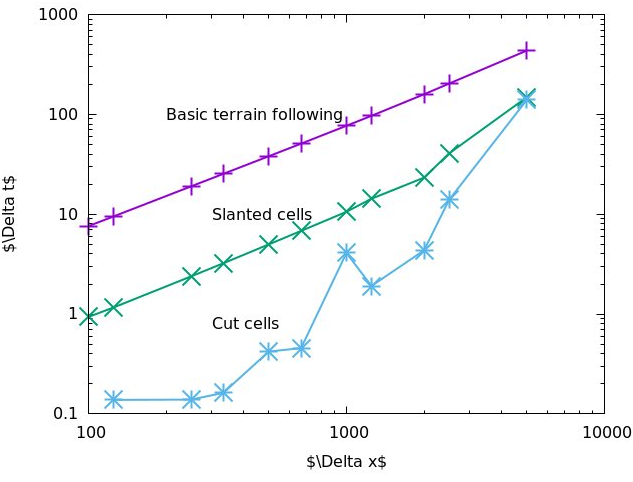
\includegraphics[width=\textwidth]{maxTimesteps.png}
	\caption{\TODO{maximum timesteps (Co=1) for BTF, slanted cells and cut cells: BTF and slanted cells scale linearly with mesh spacing, cut cells do not}}
\end{figure}

\begin{figure}
	\caption{\TODO{error fields for BTF, slanted cells and cut cells at a given mesh spacing, showing errors generated over slopes and advected downstream on slanted cell and cut cell meshes}}
\end{figure}

\begin{figure}
	\includegraphics{../fig-thermalAdvection-convergence/fig-thermalAdvection-convergence.pdf}
	\caption{\TODO{thermal advection l2 and linf convergence plots comparing BTF, slanted cells and cut cells, cubicUpwindCPCFit and linearUpwind}}
\end{figure}

\subsection{Resting atmosphere over Alpine/Andean terrain}

\subsection{Deformational flow}
Following \citep{lauritzen2012}.  Tests on hex and triangular meshes, again comparing cubicUpwindCPCFit against linearUpwind.  \citet{lauritzen2012} had six classes of test:
\begin{enumerate}
	\item \textbf{convergence tests with Gaussian hills}
	\item \textbf{minimal resolution test with cosine bell}
	\item filament preservation
	\item \textbf{"rough" distribution with a slotted cylinder}
	\item correlation preservation
	\item cosine bell in divergent flow
\end{enumerate}
I think we should reproduce a subset of these: 1, 2 and 4 would be good, perhaps 6.  But I think 3 and 5 go beyond the capabilities of our scheme and there's no need to attempt them.

\begin{figure}
	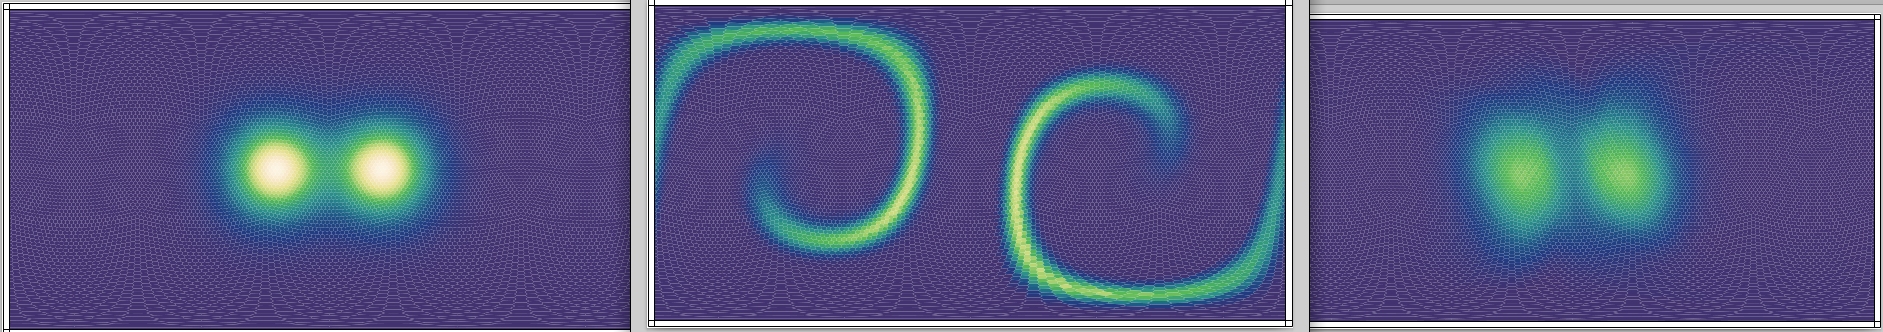
\includegraphics[width=\textwidth]{hexCubUpEvolution.png}
	\caption{\TODO{evolution of deformational flow test case with plots at $t=0$, $t=T/2$ and $t=T$.  The analytic solution at $t=T$ is identical to the initial condition.  This figure is supposed to give a sense of what `should' happen, so plot at a high resolution using whichever mesh gives better results.}}
\end{figure}

\begin{figure}
	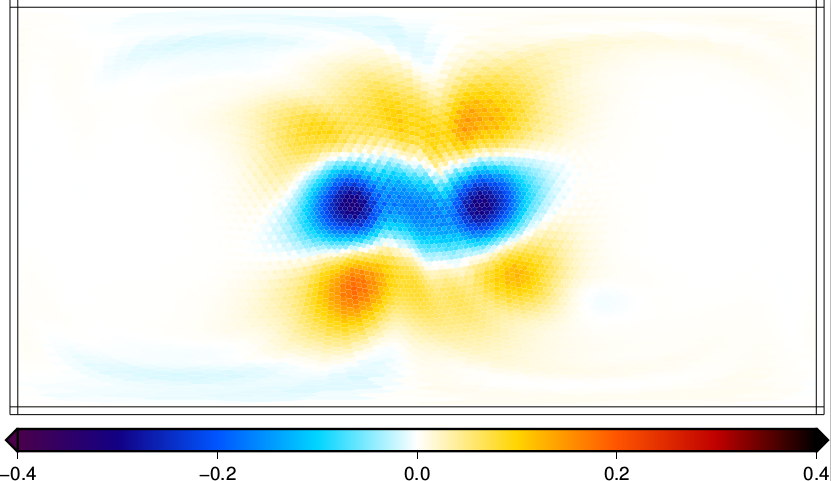
\includegraphics[width=0.5\textwidth]{hexError.png}
	\caption{\TODO{deformational flow error fields at $t=T$, comparing hex and tri meshes, linearUpwind and cubicUpwindCPCFit.  Show at the `minimal' resolution as defined by \citet{lauritzen2012}.}}
\end{figure}

% what do other people plot/analyse when they do this test?
% lauritzen2014 plot T/2 for the slotted cylinder at 1.5 and 0.75 degrees
% I think that the error field at T would be more revealing

\section{Conclusions}

The slanted cell method
\begin{itemize}
	\item alleviates the small cell problem
	\item has a linear relationship between mesh spacing and maximum timestep because arbitrarily small cells are not created
	\item accurately represents a hydrostatically balanced atmosphere at rest over steep Alpine terrain
	\item is straightforward to construct compared to the cut cell method
	\item generalises to 3D, applicable to any horizontal mesh structure
\end{itemize}

The advection scheme is
\begin{itemize}
	\item suitable for complex flows on arbitrary meshes
	\item computationally cheap at runtime, with more expensive computations depending only on the mesh geometry
	\item fourth-order convergent at best, first-order convergent at worst
	\item stable for Courant numbers up to 1
\end{itemize}

Idealised atmospheric flows over steep slopes are accurately represented using the multidimensional advection scheme without severely constraining the timestep.  The multidimensional advection scheme is suitable for complex flows on arbitrary meshes.

\section{Acknowledgements}
\TODO{Supervisors, funding bodies.  ASAM group for the mesh generator---I should ask permission to use cut cell meshes in this paper.  Dr Tristan Pryer.  Dr Shing Hing Man.}

\bibliographystyle{ametsoc2014}
\bibliography{references}

\section*{Appendix A: One-dimensional von Neumann stability analysis}
Two analyses are performed in order to find stability constraints on the weights $\mathbf{w} = \mathbf{\tilde{b}_1^+} \cdot \mathbf{m}$ as appear in equation~\eqref{eqn:weightedPinv}.  The first analysis uses two points to derive separate constraints on the upwind weight $w_u$ and downwind weight $w_d$.  The second analysis uses three points to derive a constraint that considers all weights in a stencil.

\subsection*{Two-point analysis}
We start with the conservation equation for a dependent variable $\phi$ that is discrete-in-space and continuous-in-time
\begin{align}
\frac{\partial \phi_j}{\partial t} &= - u \frac{\phi_R - \phi_L}{\Delta x} \label{eqn:advectionLR} \\
%
\intertext{where the left and right fluxes, $\phi_L$ and $\phi_R$, are weighted averages of the neighbouring points.  Assuming that $u$ is positive}
%
\phi_L &= \alpha_u \phi_{j-1} + \alpha_d \phi_j \\
\phi_R &= \beta_u \phi_j + \beta_d \phi_{j+1}
\end{align}
where $\alpha_u$ and $\beta_u$ are the upwind weights and $\alpha_d$ and $\beta_d$ are the downwind weights for the left and right fluxes respectively, and $\alpha_u + \alpha_d = 1$ and $\beta_u + \beta_d = 1$.  A subscript $j$ denotes the value at a given point $x = j \Delta x$ where $\Delta x$ is a uniform mesh spacing.

At a given time $t = n \Delta t$ at time-level $n$ and with a time-step $\Delta t$, we assume a wave-like solution with an amplification factor $A$, such that
\begin{align}
	\phi_j^{(n)} &= A^n e^{\iu j k \Delta x} \label{eqn:vn}
\end{align}
where $\phi_j^{(n)}$ denotes a value of $\phi$ at position $j$ and time-level $n$.  Using this to rewrite the left-hand side of equation~\eqref{eqn:advectionLR}
\begin{align}
\frac{\partial \phi_j}{\partial t} &= \frac{\partial}{\partial t} \left( A^{t / \Delta t} \right) e^{ijk\Delta x} = \frac{\ln A}{\Delta t} A^n e^{ikj\Delta x} \\
%
\shortintertext{hence equation~\eqref{eqn:advectionLR} becomes}
%
\frac{\ln A}{\Delta t} &= - \frac{u}{\Delta x} \left( \beta_u + \beta_d e^{ik\Delta x} - \alpha_u e^{-ik\Delta x} - \alpha_d \right) \\
\ln A &= -c \left( \beta_u - \alpha_d + \beta_d \cos k\Delta x + \iu \beta_d \sin k \Delta x - \alpha_u \cos k\Delta x + \iu \alpha_u \sin k\Delta x \right)
%
\intertext{where the Courant number $c = u \Delta t / \Delta x$.
Let $\Re = \beta_u - \alpha_d + \beta_d \cos k\Delta x - \alpha_u \cos k\Delta x$ and
$\Im = \beta_d \sin k \Delta x + \alpha_u \sin k\Delta x$, then}
%
\ln A &= -c \left( \Re + \iu \Im \right) \\
A &= e^{-c \Re} e^{-\iu c \Im} \\
%
\shortintertext{and the complex modulus of $A$ is}
%
|A| &= e^{-c \Re} = \exp \left( -c \left( \beta_u - \alpha_d + \left(\beta_d - \alpha_u \right) \cos k\Delta x \right) \right) \text{ .}
\end{align}
For stability we need $|A| \leq 1$ and, imposing the additional constraints that $\alpha_u = \beta_u$ and $\alpha_d = \beta_d$, then
\begin{align}
\left( \alpha_u - \alpha_d \right) \left( 1 - \cos k\Delta x \right) &\geq 0 \quad \forall k\Delta x
%
\shortintertext{and, given $0 \leq 1 - \cos k \Delta x \leq 2$, then}
%
\alpha_u - \alpha_d \geq 0 \text{ .} \label{eqn:twopoint-lower}
\end{align}
Additionally, we do not want more damping than a first-order upwind scheme (where $\alpha_u = \beta_u = 1$, $\alpha_d = \beta_d = 0$), having an amplification factor, $A_\mathrm{up}$, so we need $|A| \geq |A_\mathrm{up}|$, hence
\begin{align}
	\exp \left( -c \left(\alpha_u - \alpha_d\right) \left( 1 - \cos k\Delta x \right) \right) &\geq \exp \left( -c \left(1 - \cos k\Delta x \right) \right) \quad \forall k\Delta x
%
\shortintertext{therefore}
%
	\alpha_u - \alpha_d &\leq 1 \text{ .} \label{eqn:twopoint-upper}
\end{align}
Now, knowing that $\alpha_u + \alpha_d = 1$ (or $\alpha_d = 1 - \alpha_u$) then, using equations~\eqref{eqn:twopoint-lower} and \eqref{eqn:twopoint-upper},
\begin{align}
	0.5 \leq \alpha_u &\leq 1 \text{,} \label{eqn:vn:upwind} \\
	0 \leq \alpha_d &\leq 0.5 \label{eqn:vn:downwind} \text{ .}
\end{align}

\subsection*{Three-point analysis}
We start again from equation~\eqref{eqn:advectionLR} but this time approximate $\phi_L$ and $\phi_R$ using three points,
\begin{align}
	\phi_L &= \alpha_{uu} \phi_{j-2} + \alpha_u \phi_{j-1} + \alpha_d \phi_j \\
	\phi_R &= \alpha_{uu} \phi_{j-1} + \alpha_u \phi_j + \alpha_d \phi_{j+1}
\end{align}
having used the same weights $\alpha_{uu}$, $\alpha_u$ and $\alpha_d$ for both left and right fluxes.
Substituting equation~\eqref{eqn:vn} into equation~\eqref{eqn:advectionLR} we find
\begin{align}
A = \exp\left( -c \left[ \alpha_{uu} \left( e^{-ik\Delta x} - e^{-2ik\Delta x} \right) + \alpha_u \left( 1 - e^{-ik\Delta x} \right) + \alpha_d \left( e^{ik\Delta x} - 1 \right) \right] \right)
%
\intertext{so that, if the complex modulus $|A| \leq 1$ then}
%
\alpha_u - \alpha_d + \left( \alpha_{uu} - \alpha_u + \alpha_d \right) \cos k\Delta x - \alpha_{uu} \cos 2k\Delta x \geq 0 \text{ .}
\end{align}
If $k\Delta x = \pi$ then $\cos k\Delta x = -1$ and $\cos 2k\Delta x = 1$ and $\alpha_u - \alpha_d \geq \alpha_{uu}$.  If $k\Delta x = \pi / 2$ then $\cos k\Delta x = 0$ and $\cos 2k\Delta x = -1$ and $\alpha_u - \alpha_d \geq -\alpha_{uu}$.  Hence we find that
\begin{align}
	\alpha_u - \alpha_d &\geq |\alpha_{uu}| \label{eqn:uuConstraint} \text{ .}
%
\intertext{When the same analysis is performed with four points, $\alpha_{uuu}$, $\alpha_{uu}$, $\alpha_u$ and $\alpha_d$, by varying $k \Delta x$ we find that equation~\eqref{eqn:uuConstraint} still holds.
We also find that the same condition holds replacing $\alpha_{uu}$ with $\alpha_{uuu}$.  Hence, we generalise equation~\eqref{eqn:uuConstraint} to find the final stability constraint}
%
	\alpha_u - \alpha_d &\geq \max_{p\:\in\:P} |\alpha_p|
\end{align}
where the peripheral cells $P$ is the set of all stencil cells except for the upwind cell and downwind cell, and $\alpha_p$ is the weight for a given peripheral cell $p$.
We hypothesise that the three stability constraints (equations~\ref{eqn:vn:upwind}, \ref{eqn:vn:downwind} and \ref{eqn:uuConstraint}) are necessary but not sufficient for a transport scheme on arbitrarily-structured meshes.


\end{document}
